%%%%%%%%%%%%%%%%%%%%%%%%%5
%% abtex2-modelo-trabalho-academico.tex, v<VERSION> laurocesar
%% Copyright 2012-<COPYRIGHT_YEAR> by abnTeX2 group at http://www.abntex.net.br/
%%
%% This work may be distributed and/or modified under the
%% conditions of the LaTeX Project Public License, either version 1.3
%% of this license or (at your option) any later version.
%% The latest version of this license is in
%%   http://www.latex-project.org/lppl.txt
%% and version 1.3 or later is part of all distributions of LaTeX
%% version 2005/12/01 or later.
%%
%% This work has the LPPL maintenance status `maintained'.
%%
%% The Current Maintainer of this work is the abnTeX2 team, led
%% by Lauro César Araujo. Further information are available on
%% http://www.abntex.net.br/
%%
%% This work consists of the files abntex2-modelo-trabalho-academico.tex,
%% abntex2-modelo-include-comandos and abntex2-modelo-references.bib
%%

% ------------------------------------------------------------------------
% ------------------------------------------------------------------------
% abnTeX2: Modelo de Trabalho Academico (tese de doutorado, dissertacao de
% mestrado e trabalhos monograficos em geral) em conformidade com
% ABNT NBR 14724:2011: Informacao e documentacao - Trabalhos academicos -
% Apresentacao
% ------------------------------------------------------------------------
% ------------------------------------------------------------------------

\documentclass[
	% -- opções da classe memoir --
	12pt,				% tamanho da fonte
%  openright,			% capítulos começam em pág ímpar (insere página vazia caso preciso)
	oneside,			% para impressão em recto e verso use twoside
	a4paper,			% tamanho do papel.
	% -- opções da classe abntex2 --
	%chapter=TITLE,		% títulos de capítulos convertidos em letras maiúsculas
	%section=TITLE,		% títulos de seções convertidos em letras maiúsculas
	%subsection=TITLE,	% títulos de subseções convertidos em letras maiúsculas
	%subsubsection=TITLE,% títulos de subsubseções convertidos em letras maiúsculas
	% -- opções do pacote babel --
	english,			% idioma adicional para hifenização
	french,				% idioma adicional para hifenização
	spanish,			% idioma adicional para hifenização
	brazil				% o último idioma é o principal do documento
	]{abntex2}

% ---
% Pacotes básicos
% ---
\usepackage{times}			    % Usa fonte times
\renewcommand{\ABNTEXchapterfont}{\normalfont} % para aplicar a fonte escolhida em tudo
\usepackage[T1]{fontenc}		% Selecao de codigos de fonte.
\usepackage[utf8]{inputenc}		% Codificacao do documento (conversão automática dos acentos)
\usepackage{lastpage}			% Usado pela Ficha catalográfica
\usepackage{indentfirst}		% Indenta o primeiro parágrafo de cada seção.
\usepackage{color}				% Controle das cores
\usepackage{graphicx}			% Inclusão de gráficos
\usepackage{microtype} 			% para melhorias de justificação
% ---

% ---
% Pacotes adicionais, usados apenas no âmbito do Modelo Canônico do abnteX2
% ---
\usepackage{lipsum}				% para geração de dummy text
% ---

% ---
% Pacotes de citações
% ---
\usepackage[brazilian,hyperpageref]{backref}	 % Paginas com as citações na bibl
\usepackage[alf]{abntex2cite}	% Citações padrão ABNT

% ---
% CONFIGURAÇÕES DE PACOTES
% ---

% ---
% Configurações do pacote backref
% Usado sem a opção hyperpageref de backref
\renewcommand{\backrefpagesname}{Citado na(s) página(s):~}
% Texto padrão antes do número das páginas
\renewcommand{\backref}{}
% Define os textos da citação
\renewcommand*{\backrefalt}[4]{
	\ifcase #1 %
		Nenhuma citação no texto.%
	\or
		Citado na página #2.%
	\else
		Citado #1 vezes nas páginas #2.%
	\fi}%
% ---

% ---
% Informações de dados para CAPA e FOLHA DE ROSTO
% ---
\titulo{Aprimoramento da ferramenta Limarka para TCCs: Funcionalidades avançadas
e guia de uso em Markdown para Estudantes Universitários}
\autor{Reinan Gabriel Dos Santos Souza}
\data{2023}
\local{Lagarto - SE}
\orientador{Nome-do-Orientador}
\coorientador{}
\instituicao{%
  Instituto Federal de Sergipe
  \par
  Sistemas de informação
}
\tipotrabalho{Monografia}

% O preambulo deve conter o tipo do trabalho, o objetivo (propósito),
% o nome da instituição e a área de concentração.
% Esse texto irá compor a Folha de Rosto e Folha de Aprovação.
\preambulo{
Trabalho de Conclusão de Curso apresentado ao Curso de Graduação em
Sistemas de Informação do Campus Lagarto do Instituto Federal de
Educação, Ciência e Tecnologia, como requisito parcial à obtenção do
grau de bacharel em Sistemas de Informação.
\newline\textbf{Área de concentração}: Computação.
}%% fim do preambulo




% ---
% Configurações de aparência do PDF final

% alterando o aspecto da cor azul
\definecolor{blue}{RGB}{41,5,195}

% informações do PDF
\makeatletter
\hypersetup{
     	%pagebackref=true,
		pdftitle={\@title},
		pdfauthor={\@author},
    	pdfsubject={\imprimirpreambulo},
	    pdfcreator={LaTeX with abnTeX2 and Limarka},
		pdfkeywords={abnt}{latex}{abntex}{abntex2}{trabalho acadêmico}{limarka},
		colorlinks=false,       		% false: boxed links; true: colored links
    	linkcolor=black,          	% color of internal links
    	citecolor=black,        		% color of links to bibliography
    	filecolor=black,      		% color of file links
		urlcolor=black,
		bookmarksdepth=4
}
\makeatother
% ---

% ---
% Possibilita criação de Quadros e Lista de quadros.
% Ver https://github.com/abntex/abntex2/issues/176
%
\newcommand{\quadroname}{Quadro}
\newcommand{\listofquadrosname}{Lista de quadros}

\newfloat[chapter]{quadro}{loq}{\quadroname}
\newlistof{listofquadros}{loq}{\listofquadrosname}
\newlistentry{quadro}{loq}{0}

% configurações para atender às regras da ABNT
\setfloatadjustment{quadro}{\centering}
\counterwithout{quadro}{chapter}
\renewcommand{\cftquadroname}{\quadroname\space}
\renewcommand*{\cftquadroaftersnum}{\hfill--\hfill}

% ---


% ---
% Espaçamentos entre linhas e parágrafos
% ---

% O tamanho do parágrafo é dado por:
\setlength{\parindent}{1.3cm}

% Controle do espaçamento entre um parágrafo e outro:
\setlength{\parskip}{0.2cm}  % tente também \onelineskip

% ---
% compila o indice
% ---
\makeindex
% ---

%---
% CONFIGURAÇÕES EXTRA DO LIMARKA
%---

% Configura citações de pandoc para 4cm à esquerda (utiliza o ambiente quote)
\renewenvironment{quote}
  {\small\list{}{\rightmargin=0.1cm \leftmargin=4cm}%
   \item\relax}
  {\endlist}

% Para incluir páginas PDF (ficha catalografica e folha de aprovação)
\usepackage[dvipsnames]{xcolor} % http://tex.stackexchange.com/questions/124636/package-xcolor-error-undefined-colors-maroon-royal-blue-when-master-has-pdf
\usepackage{pdfpages}
\usepackage{longtable,ltcaption,booktabs} % para as tabelas pandoc e quadros ABNT
%\usepackage{floatrow}
%\floatsetup[figure]{capposition=top}

% Para melhorar o visual do quadro
\usepackage{boldline} 
\def\toprule{\hlineB{3}} % primeira linha mais gorda
\def\midrule{\hline}
\def\bottomrule{\hlineB{3}} % última linha mais gorda



% ---
% BUG: Imagens e tabelas apareciam no meio da página em branco
% https://github.com/abntex/trabalho-academico-limarka/issues/1
% O código a seguir posta imagens ou tabelas em página em branco no topo, em vez do meio (comportamento padrão)
\makeatletter
\setlength{\@fptop}{5pt} % Set distance from top of page to first float
\makeatother
% ---

% ---
% Usado pelo limarka como hook para criação de novas listas.
% https://github.com/abntex/trabalho-academico-limarka/issues/16
%
\newcommand{\listasdousuario}{}

% ---
% CUSTOMIZAÇÕES DO USUÁRIO (somente se existir arquivo config/latexcustomizacao.sty)
% ---
\IfFileExists{latexcustomizacao.sty}{\usepackage{latexcustomizacao}}{}

%%
%% Esse modelo é responsável pela impressão dos seguintes elementos:
%% Capa, Folha de rosto e Ficha catalográfica.

\special{dvipdfmx:config z 0}

% ----
% Início do documento
% ----
\begin{document}

% Seleciona o idioma do documento (conforme pacotes do babel)
%\selectlanguage{english}
\selectlanguage{brazil}

% Retira espaço extra obsoleto entre as frases.
\frenchspacing

% ----------------------------------------------------------
% ELEMENTOS PRÉ-TEXTUAIS
% ----------------------------------------------------------
% \pretextual

% ---
% Capa 
% ---
% Gerando capa abnTeX2
\imprimircapa

% ---

% ----------------------------------------------------------
% ELEMENTOS PRÉ-TEXTUAIS
% ----------------------------------------------------------
% \pretextual

% ---
% Folha de rosto: sempre será impressa
% ---
\imprimirfolhaderosto

% ---
% Sem ficha catalográfica
% ---
% ---


% ---
% ERRATA: Sem errata
% ---


% ---
% Sem Folha de aprovação
% ---
% ---
% ---
% Dedicatória
% ---
% ---
% Agradecimentos
% ---
\begin{agradecimentos}

Gostaria de expressar meus mais sinceros agradecimentos aos estimados
professores do Instituto Federal de Educação, Ciência e Tecnologia de
Sergipe (IFS). Este trabalho de conclusão de curso não teria sido
possível sem a orientação, o apoio e a sabedoria que vocês generosamente
compartilharam ao longo da minha jornada acadêmica.

Suas aulas inspiradoras, seu compromisso com a excelência educacional e
seu incentivo constante foram fundamentais para o meu desenvolvimento
acadêmico e pessoal. Cada um de vocês desempenhou um papel fundamental
no meu crescimento como estudante e na minha capacidade de enfrentar os
desafios acadêmicos.

Este trabalho é uma celebração do aprendizado e da dedicação que
testemunhei no IFS. Agradeço sinceramente a todos os professores que
fizeram parte desta jornada, contribuindo para o meu crescimento
acadêmico e pessoal.

\end{agradecimentos}
% ---
% ---
% Epígrafe
% ---
% ---

% ---
% Resumo na língua vernácula (obrigatório)
% ---


% resumo em português
\setlength{\absparsep}{18pt} % ajusta o espaçamento dos parágrafos do resumo
\begin{resumo}

  Este trabalho de pesquisa concentra-se na aprimoração da ferramenta
  Limarka, destinada à elaboração de Trabalhos de Conclusão de Curso
  (TCCs) em formato Markdown. Além disso, o estudo aborda a criação de
  documentação abrangente que visa destacar e facilitar o uso efetivo
  dessa ferramenta. O objetivo principal é melhorar a experiência dos
  estudantes na elaboração de TCCs, proporcionando uma ferramenta mais
  eficaz e fornecendo orientações detalhadas por meio da documentação. Ao
  unir esses esforços de aprimoramento e documentação, busca-se
  simplificar o processo de criação de TCCs em Markdown, tornando-o mais
  acessível e eficiente para os acadêmicos.

 \textbf{Palavras-chave}: Limarka, Markdown, Melhoria, TCCs, Ferramenta, Aprimoramento e
Produtividade
\end{resumo}


% ---
% Resumo em língua estrangeira (obrigatório)
% ---

% resumo em inglês
\begin{resumo}[Abstract]
 \begin{otherlanguage*}{english}
   This research work focuses on improving the Limarka tool, designed for
   preparing Course Completion Papers (TCCs) in Markdown format.
   Furthermore, the study addresses the creation of comprehensive
   documentation that aims to highlight and facilitate the effective use of
   this tool. The main objective is to improve students' experience in
   preparing TCCs, providing a more effective tool and providing detailed
   guidance through documentation. By combining these improvement and
   documentation efforts, we seek to simplify the process of creating TCCs
   in Markdown, making it more accessible and efficient for academics.

   \vspace{\onelineskip}
 
   \noindent 
   \textbf{Keywords}: Limarka, Markdown, Improvement, TCCs, Tool, Improvement and Productivity
 \end{otherlanguage*}
\end{resumo}


% ---

% ---
% Lista de ilustrações (opcional): não utilizando.
% ---


% ---
% Lista de quadros (opcional): não utilizando.
% ---

% Carrega listas definidas pelo usuário em `latexcustomizacao.sty`
\listasdousuario
% ---
% Lista de tabelas (opcional): não utilizando
% ---

% ---
% Lista de abreviaturas e siglas (opcional)
% ---
\begin{siglas}
  \item[ABNT] Associação Brasileira de Normas Técnicas
  \item[TCC] Trabalho de Conclusão de Curso
  \item[BSI] Bacharelado em Sistemas de Informação
\end{siglas}
% ---

% ---
% Lista de símbolos (opcional): AUSENTE
% ---
% ---
% Sumário
% ---
\pdfbookmark[0]{\contentsname}{toc}
\tableofcontents*
\cleardoublepage
% ---


% ----------------------------------------------------------
% ELEMENTOS TEXTUAIS
% ----------------------------------------------------------
\textual
\pagestyle{simple}                  % #17 Cabeçalho apenas com
\aliaspagestyle{chapter}{simple}    % a numeração das páginas


\hypertarget{introduuxe7uxe3o}{%
\chapter{Introdução}\label{introduuxe7uxe3o}}

\hypertarget{justificativa}{%
\chapter{Justificativa}\label{justificativa}}

A elaboração de trabalhos de conclusão de curso (TCCs) representa uma
etapa fundamental na jornada acadêmica dos estudantes de graduação,
exigindo a aplicação de conhecimentos adquiridos ao longo do curso e a
produção de um documento formal que atenda a rigorosos padrões
acadêmicos. Neste contexto, a ferramenta Limarka emerge como uma solução
inovadora para a elaboração de TCCs em formato Markdown, prometendo uma
abordagem mais simplificada e eficiente em comparação com os editores de
texto tradicionais. No entanto, a adoção da ferramenta Limarka ainda
enfrenta desafios significativos, principalmente devido à falta de
documentação abrangente e suporte para as necessidades específicas dos
estudantes do curso de Bacharelado em Sistemas de Informação do
Instituto Federal de Sergipe (IFS), Campus Lagarto.

Este trabalho justifica-se pela necessidade premente de superar esses
obstáculos, aprimorando a ferramenta Limarka para torná-la mais
acessível, intuitiva e adaptada às especificidades dos padrões
acadêmicos brasileiros, em especial às normas da ABNT. Além disso, a
elaboração de documentação detalhada e orientada ao usuário visa equipar
os estudantes com os recursos necessários para aproveitar plenamente os
benefícios da escrita em Markdown, otimizando o processo de elaboração
de TCCs.

A importância deste estudo é evidenciada pelo potencial de transformar
significativamente a experiência de escrita acadêmica dos estudantes,
permitindo uma maior concentração no conteúdo científico em detrimento
das preocupações com a formatação do documento. Ao facilitar o acesso e
a utilização da ferramenta Limarka, espera-se não apenas melhorar a
eficiência e a qualidade dos trabalhos produzidos, mas também incentivar
a adoção de práticas de escrita colaborativa e a utilização de
tecnologias abertas e acessíveis no ambiente acadêmico.

A contribuição deste trabalho estende-se para além dos limites do IFS,
Campus Lagarto, uma vez que as melhorias implementadas na ferramenta
Limarka e a documentação produzida podem servir como referência para
outras instituições de ensino superior que buscam inovar nas
metodologias de elaboração de TCCs. Desta forma, este TCC não apenas
atende a uma demanda específica do curso de Bacharelado em Sistemas de
Informação, mas também contribui para o avanço das práticas de escrita
científica no contexto acadêmico brasileiro, promovendo a inclusão
digital e a democratização do acesso a ferramentas educacionais de
qualidade.

Portanto, o aprimoramento da ferramenta Limarka e a criação de uma
documentação detalhada e acessível representam passos importantes na
direção de um ensino superior mais inovador, eficiente e inclusivo,
alinhado às demandas contemporâneas por tecnologias educacionais que
facilitam a produção de conhecimento científico e sua disseminação.

\hypertarget{objetivo}{%
\chapter{Objetivo}\label{objetivo}}

Nesta seção, serão é apresentado o objetivo geral e os objetivos
específicos desta pesquisa.

\hypertarget{objetivo-geral}{%
\section{Objetivo Geral}\label{objetivo-geral}}

O objetivo geral deste trabalho é construir um ecossistema, com manual
de instruções, para a ferramenta Lamarka que permita a escrita de
trabalhos cientificos de forma mais acessível e eficaz pelos os
estudantes do curso de Bacharelado em Sistemas de Informação (BSI) do
IFS Campus Lagarto.

\hypertarget{objetivos-especuxedficos}{%
\section{Objetivos Específicos}\label{objetivos-especuxedficos}}

A fim de atingir o objetivo geral, são definidos os seguintes objetivos
específicos:

\begin{itemize}
\tightlist
\item
  \textbf{Disponibilizar o Lamarka por meio de um ambiente Docker}:
  Facilitar o acesso e a instalação da ferramenta, tornando-a disponível
  em um ambiente Docker de fácil configuração;
\item
  \textbf{Desenvolver uma ferramenta de linha de comando}: Criar
  comandos que simplifiquem o processo de construção de documentos em
  Markdown usando o Lamarka;
\item
  \textbf{Implementar um pipeline no Github Actions}: Estabelecer uma
  estrutura de pipeline automatizado para compilar projetos Lamarka de
  maneira eficiente no GitHub;
\item
  \textbf{Habilitar exportação para HTML no Github Pages}: Aprimorar a
  capacidade do Lamarka de exportar documentos em Markdown para o
  formato HTML, tornando-os acessíveis no Github Pages;
\item
  \textbf{Integrar funcionalidade de importação de arquivos markdown}:
  Adicionar a capacidade de importar documentos Markdown existentes,
  simplificando o processo de compilação do Lamarka;
\item
  \textbf{Reestruturar a organização de arquivos do template}: Melhorar
  a estrutura de arquivos do template para torná-lo mais intuitivo e
  adequado aos padrões do IFS Campus Lagarto;
\item
  \textbf{Conduzir testes rigorosos}: Realizar testes rigorosos para
  garantir que as melhorias no Lamarka atendam às necessidades dos
  estudantes, garantindo sua eficácia;
\item
  \textbf{Produzir uma documentação abrangente}: Criar uma documentação
  detalhada, abrangendo desde a instalação até a formatação de
  documentos em conformidade com os padrões do IFS Campus Lagarto;
\item
  \textbf{Promover a adoção e divulgação}: Incentivar ativamente a
  utilização da ferramenta aprimorada e da documentação entre os
  estudantes do curso de BSI, buscando uma ampla adoção do Lamarka como
  ferramenta eficaz para a elaboração de TCCs no IFS;
\item
  \textbf{Avaliar o impacto das melhorias}: Realizar uma análise crítica
  para avaliar o impacto das melhorias no Lamarka na eficiência e na
  qualidade da produção de TCCs, coletando feedback dos usuários e
  ajustando a ferramenta conforme necessário.
\end{itemize}

\hypertarget{organizauxe7uxe3o-da-proposta}{%
\section{Organização da Proposta}\label{organizauxe7uxe3o-da-proposta}}

\hypertarget{fundamentauxe7uxe3o-teuxf3rica}{%
\chapter{Fundamentação Teórica}\label{fundamentauxe7uxe3o-teuxf3rica}}

\hypertarget{metodologia}{%
\chapter{Metodologia}\label{metodologia}}

Nesta seção, serão é apresentado a metodologia deste trabalho.

\hypertarget{abordagem-da-pesquisa}{%
\section{Abordagem da pesquisa}\label{abordagem-da-pesquisa}}

Este trabalho adota uma abordagem de pesquisa aplicada, focada no
desenvolvimento e na avaliação de uma solução tecnológica destinada a
facilitar a elaboração de trabalhos de conclusão de curso (TCCs) em
formato Markdown. O objetivo é desenvolver melhorias na ferramenta
Limarka, assim como documentar seu uso de forma efetiva, visando
otimizar a experiência dos usuários, principalmente estudantes do curso
de Bacharelado em Sistemas de Informação. A metodologia é composta por
etapas de planejamento, desenvolvimento, teste e avaliação, seguindo
princípios da engenharia de software.

\hypertarget{desenvolvimento-da-ferramenta}{%
\section{Desenvolvimento da
ferramenta}\label{desenvolvimento-da-ferramenta}}

Para atender aos objetivos específicos propostos, o desenvolvimento da
ferramenta será realizado em etapas, iniciando com a configuração de um
ambiente Docker para facilitar o acesso e a instalação da ferramenta
Limarka. Em seguida, será desenvolvida uma interface de linha de comando
para simplificar a criação e a compilação de documentos Markdown. A
implementação de um pipeline automatizado no GitHub Actions será
realizada para permitir a compilação eficiente de projetos Limarka. Além
disso, serão implementadas funcionalidades para exportação de documentos
para HTML via GitHub Pages e para importação de arquivos Markdown
existentes.

\hypertarget{estratuxe9gias-de-teste}{%
\section{Estratégias de teste}\label{estratuxe9gias-de-teste}}

Para garantir a qualidade e a eficácia das melhorias implementadas,
serão conduzidos testes rigorosos em cada etapa do desenvolvimento.
Esses testes incluirão testes unitários para validar funcionalidades
individuais, testes de integração para assegurar que os componentes da
ferramenta trabalhem conjuntamente de forma eficiente e testes de
usabilidade para avaliar a experiência do usuário.

\hypertarget{documentauxe7uxe3o}{%
\section{Documentação}\label{documentauxe7uxe3o}}

Uma parte crucial deste trabalho é a produção de documentação
abrangente, que cobrirá desde a instalação da ferramenta e configuração
do ambiente até a utilização efetiva da mesma para a elaboração de TCCs.
A documentação será estruturada de maneira clara e acessível, visando
facilitar o uso da ferramenta por parte dos estudantes e docentes.

\hypertarget{avaliauxe7uxe3o-e-feedback}{%
\section{Avaliação e feedback}\label{avaliauxe7uxe3o-e-feedback}}

Após a implementação das melhorias e da documentação, será realizada uma
avaliação do impacto dessas mudanças na eficiência e qualidade da
elaboração de TCCs. Essa avaliação contará com a coleta de feedback de
usuários reais da ferramenta, incluindo estudantes e professores. Os
resultados dessa avaliação serão utilizados para realizar ajustes finais
na ferramenta e na documentação, garantindo que as necessidades dos
usuários sejam plenamente atendidas.

\hypertarget{desenvolvimento-das-melhorias}{%
\chapter{Desenvolvimento das
melhorias}\label{desenvolvimento-das-melhorias}}

Para garantir que a ferramenta Limarka atendesse às necessidades dos
alunos de maneira mais eficaz, foram implementadas diversas melhorias.
Essas melhorias visaram aprimorar a estrutura do projeto, facilitar a
configuração e o uso da ferramenta, além de integrar novas
funcionalidades que aumentassem a eficiência no desenvolvimento de
trabalhos acadêmicos. A seguir, detalhamos os principais aprimoramentos
realizados.

\hypertarget{fork-e-melhorias-no-template}{%
\section{Fork e melhorias no
Template}\label{fork-e-melhorias-no-template}}

Com o objetivo de aprimorar a ferramenta Limarka, realizei o fork do
projeto
\href{https://github.com/abntex/trabalho-academico-limarka}{abntex/trabalho-academico-limarka},
criando o repositório
\href{https://github.com/ReinanHS/limarka-template-tcc}{limarka-template-tcc}
no GitHub. Essa ação foi motivada pela necessidade de melhorar o modelo
original e adicionar novas funcionalidades que pudessem ajudar os alunos
a escreverem seus trabalhos acadêmicos com maior facilidade.

\hypertarget{organizauxe7uxe3o-da-estrutura-de-pastas}{%
\subsection{Organização da estrutura de
pastas}\label{organizauxe7uxe3o-da-estrutura-de-pastas}}

A estrutura de pastas original do modelo
\texttt{abntex/trabalho-academico-limarka} era funcional, mas
apresentava algumas limitações em termos de organização e facilidade de
uso. No fork \texttt{limarka-template-tcc}, reorganizei as pastas de
forma a tornar o projeto mais intuitivo para os usuários. Agora, os
arquivos são distribuídos em diretórios específicos para cada tipo de
conteúdo, como páginas, compilações, configurações e imagens,
facilitando a navegação pelo projeto e a localização de arquivos
específicos.

Veja a estrutura de cada diretório e suas respectivas funções:

\begin{itemize}
\tightlist
\item
  \textbf{.devcontainer}: Define o ambiente de desenvolvimento baseado
  em contêiner, facilitando a configuração em diferentes máquinas;
\item
  \textbf{.github}: Inclui recursos importantes como templates para
  issues e pull requests, além de guias para contribuição;
\item
  \textbf{.vscode}: Armazena configurações recomendadas para usuários do
  VS Code, como extensões e preferências de formatação;
\item
  \textbf{build}: Diretório destinado aos outputs do processo de build,
  como PDFs gerados a partir do Markdown;
\item
  \textbf{config}: Contém arquivos de configuração que determinam o
  comportamento de várias partes do projeto, como parâmetros de
  compilação;
\item
  \textbf{docs}: Hospeda a documentação do projeto, que pode incluir
  manuais do usuário, especificações técnicas e guias de instalação;
\item
  \textbf{imagens}: Repositório para as imagens utilizadas no documento,
  ajudando a organizar os recursos visuais;
\item
  \textbf{pages}: Diretório que contém os arquivos markdown utilizados
  no documento;
\item
  \textbf{templates}: Armazena os templates LaTeX que definem a
  aparência e estrutura do documento final.
\end{itemize}

Graças a essa reorganização, colaboradores e usuários que buscam
modificar, personalizar ou contribuir para o projeto encontrarão uma
estrutura mais organizada e moderna em comparação a vários repositórios
existentes no GitHub. Isso possibilita a configuração de diversos
recursos dentro do projeto.

\hypertarget{criauxe7uxe3o-do-diretuxf3rio-.vscode}{%
\subsection{Criação do diretório
.vscode}\label{criauxe7uxe3o-do-diretuxf3rio-.vscode}}

A criação deste diretório permitiu adicionar várias configurações que
facilitam o uso do projeto no Visual Studio Code, uma das ferramentas
sugeridas na documentação para trabalhar com este repositório. Dentro
deste diretório, foram configurados snippets, tasks e a sugestão de
instalação de extensões que se integram ao projeto, facilitando a
escrita dos trabalhos acadêmicos.

Quando o usuário abre o editor, essas configurações são automaticamente
importadas, e as extensões necessárias são sugeridas para instalação. A
Figura \ref{extensoes_mapeadas_vscode} demonstra como a sugestão é
apresentada aos alunos ao abrirem o projeto no VSCode:

\begin{figure}[htbp]
\hypertarget{extensoes_mapeadas_vscode}{%
\caption{Exemplificação da recomendação de instalação de extensões no VSCode}\label{extensoes_mapeadas_vscode}
\begin{center}
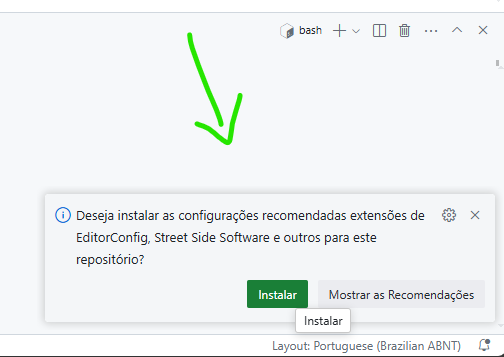
\includegraphics[scale=0.6]{imagens/screenshot/extensoes-mapeadas-vscode.png}
\end{center}
}
\legend{Fonte: Autor.}
\end{figure}

As extensões mapeadas foram escolhidas por sua utilidade na escrita de
documentos em Markdown, como a extensão \textbf{Brazilian
Portuguese - Code Spell Checker}, responsável por corrigir erros de
ortografia e concordância, e a extensão \textbf{Markdown Table
Formatter}, que auxilia na criação e formatação de tabelas de forma
correta e integrada aos snippets.

Outro detalhe importante adicionado ao modelo original é a configuração
de uma task para realizar o build do documento pelo Limarka. No modelo
original, os alunos precisariam digitar alguns comandos no terminal para
compilar as informações no formato PDF. No entanto, isso poderia gerar
um esforço adicional para o aluno, desviando seu foco da tarefa
principal, que é a escrita do documento.

Para solucionar esse problema, foi criada uma configuração de task no
VSCode, permitindo que a compilação do documento seja executada através
de atalhos ou pressionando um botão na interface do VSCode. Essa
configuração simplifica significativamente o processo de compilação,
tornando-o mais acessível e permitindo que os alunos se concentrem na
elaboração do conteúdo do seu trabalho acadêmico. A Figura
\ref{limarka_builder_task} demonstra o processo de execução da task pela
interface do VSCode:

\begin{figure}[htbp]
\hypertarget{limarka_builder_task}{%
\caption{Exemplificação da execução da task de build para o Limarka}\label{limarka_builder_task}
\begin{center}
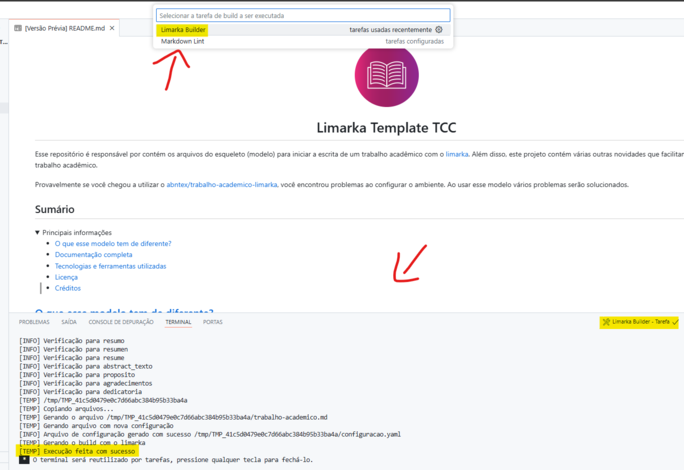
\includegraphics[scale=0.6]{imagens/screenshot/limarka-builder-task.png}
\end{center}
}
\legend{Fonte: Autor.}
\end{figure}

Ao abrir a tela de tasks, que pode ser encontrada através do painel de
terminal, o aluno encontrará uma lista de jobs disponíveis para execução
dentro do editor. Utilizando as configurações do modelo disponibilizado,
o aluno verá uma job chamada \textbf{Limarka Builder}. Ao selecionar
essa opção, um terminal será aberto e todo o fluxo de build do documento
será exibido, incluindo a geração do PDF. Caso ocorra algum erro, o
aluno poderá visualizar as informações de erro diretamente no painel ou
através dos logs armazenados na pasta de build.

\hypertarget{criauxe7uxe3o-do-diretuxf3rio-build}{%
\subsection{Criação do diretório
build}\label{criauxe7uxe3o-do-diretuxf3rio-build}}

Foi criada uma pasta exclusiva para a compilação dos resultados da
ferramenta Limarka, separando os arquivos de build dos arquivos
principais do projeto. Anteriormente, as informações de compilação
ficavam na raiz do projeto, o que causava confusão. Com um diretório
dedicado, todas as saídas de compilação são organizadas em um único
local, melhorando a clareza e a manutenção do projeto. As vantagens de
ter um diretório separado para compilação incluem:

\begin{itemize}
\tightlist
\item
  Facilita a limpeza e reconstrução do projeto sem interferir nos
  arquivos de origem;
\item
  Melhora a organização, tornando mais fácil identificar e resolver
  problemas de build;
\item
  Simplifica a integração com ferramentas de CI/CD, que podem focar
  diretamente no diretório de build.
\end{itemize}

\hypertarget{criauxe7uxe3o-do-diretuxf3rio-.github}{%
\subsection{Criação do diretório
.github}\label{criauxe7uxe3o-do-diretuxf3rio-.github}}

Este diretório foi criado para adicionar as configurações do
\href{https://docs.github.com/pt/actions}{GitHub Actions}, integrando o
projeto com pipelines de CI/CD. A integração com CI/CD é crucial para
automatizar testes, builds e deploys, garantindo que o documento esteja
sempre em um estado funcional. Além disso, centraliza templates de
issues e pull requests, facilitando a contribuição e a manutenção do
projeto.

\hypertarget{criauxe7uxe3o-do-diretuxf3rio-.devcontainer}{%
\subsection{Criação do diretório
.devcontainer}\label{criauxe7uxe3o-do-diretuxf3rio-.devcontainer}}

O diretório \texttt{.devcontainer} foi criado para configurar o
\href{https://docs.github.com/pt/codespaces/overview}{GitHub
Codespaces}. Esta configuração permite que os usuários desenvolvam e
testem o projeto em um ambiente pré-configurado diretamente no
navegador, eliminando a necessidade de configuração local. Isso
proporciona uma experiência de desenvolvimento consistente e reduz
problemas de compatibilidade entre diferentes ambientes de
desenvolvimento.

\hypertarget{criauxe7uxe3o-do-diretuxf3rio-pages}{%
\subsection{Criação do diretório
pages}\label{criauxe7uxe3o-do-diretuxf3rio-pages}}

Este diretório foi criado para organizar arquivos específicos do
projeto, como introduções e anexos. Além disso, serve para a compilação
de páginas que são publicadas em um site estático no GitHub Pages pelo
\href{https://github.com/ReinanHS/limarka-render-html}{limarka-render-html},
uma ferramenta desenvolvida para melhorar ainda mais a estrutura
original do projeto. Com essa ferramenta, é possível compilar as
informações em formato HTML, permitindo que sejam publicadas na internet
e acessadas de maneira fácil.

A ferramenta \texttt{limarka-render-html} coleta as informações
presentes no diretório \texttt{pages} seguindo regras estabelecidas no
arquivo de configuração do projeto. Durante o processo de compilação no
CI/CD, ela também realiza a compilação dessas informações em formato
HTML.

\begin{figure}[htbp]
\hypertarget{limarka_template_tcc_html}{%
\caption{Exemplificação da página em HTML gerada pela ferramenta}\label{limarka_template_tcc_html}
\begin{center}
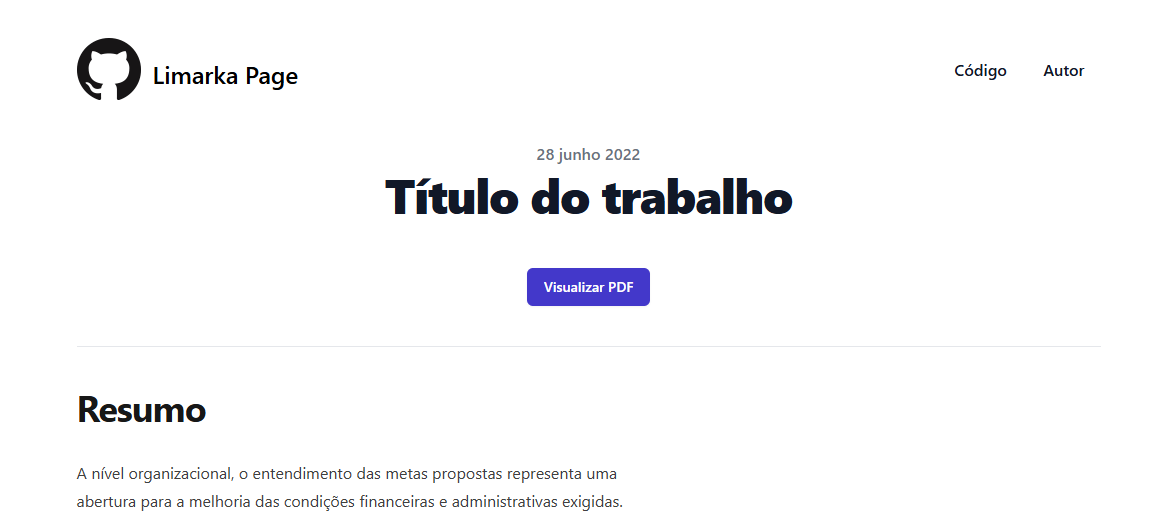
\includegraphics[scale=0.4]{imagens/screenshot/limarka-template-tcc-html.png}
\end{center}
}
\legend{Fonte: Autor.}
\end{figure}

Observando a figura \ref{limarka_template_tcc_html}, podemos ver que a
ferramenta faz o mapeamento do arquivo de configuração do projeto,
extraindo informações como título, aluno, orientador e outros dados
necessários para exibir um contexto geral sobre o documento. Além disso,
a ferramenta disponibiliza um link para a visualização do documento
compilado em PDF.

Ao utilizar a compilação nesse formato e a publicação na internet, os
alunos conseguem compartilhar facilmente os resultados de seu trabalho
com orientadores ou qualquer outra pessoa com acesso à internet. Isso
permite que o trabalho do aluno seja visualizado diretamente pela
internet, sem a necessidade de compilar as informações ou configurar o
projeto em um computador local, uma vez que as informações estão
publicamente disponíveis online.

O aluno também pode configurar a ferramenta para decidir se deseja ou
não publicar as informações na internet. Dependendo das necessidades do
aluno e de sua preferência quanto à exposição de seu trabalho, a
publicação pode ser habilitada ou desabilitada nas configurações do
CI/CD.

\hypertarget{criauxe7uxe3o-do-diretuxf3rio-docs}{%
\subsection{Criação do diretório
docs}\label{criauxe7uxe3o-do-diretuxf3rio-docs}}

Este diretório foi criado para seguir a filosofia ``\emph{documentação
como código}'' (docs as code). Nele, toda a documentação da ferramenta é
mantida, incluindo manuais do usuário, especificações técnicas e guias
de instalação. Os benefícios do docs as code incluem:

\begin{itemize}
\tightlist
\item
  Manutenção da documentação atualizada junto com o código, garantindo
  que as informações estejam sempre corretas e relevantes;
\item
  Facilidade de contribuição, permitindo que desenvolvedores atualizem a
  documentação junto com as mudanças de código;
\item
  Centralização de informações, tornando mais fácil para os usuários
  encontrar e entender as funcionalidades da ferramenta.
\end{itemize}

\hypertarget{implementauxe7uxe3o-da-funcionalidade-de-importauxe7uxe3o-de-arquivos-em-markdown}{%
\section{Implementação da funcionalidade de importação de arquivos em
Markdown}\label{implementauxe7uxe3o-da-funcionalidade-de-importauxe7uxe3o-de-arquivos-em-markdown}}

Com as melhorias na organização da estrutura de pastas, surgiu a
necessidade de dividir o documento dentro dessa nova organização. No
modelo original, o documento era escrito a partir do arquivo
\texttt{trabalho-academico.md}, que continha todas as informações do
documento a ser processado pela ferramenta Limarka. Dessa forma, os
alunos precisavam escrever todo o conteúdo de seu TCC em um único
arquivo, o que podia ser desorganizado e difícil de gerenciar.

No entanto, foi adicionada uma nova funcionalidade que realiza uma
pré-compilação deste arquivo, possibilitando que os alunos façam a
importação de outros arquivos em Markdown. Com essa nova estratégia, os
alunos podem ter um arquivo separado para cada parte do seu documento,
como um arquivo apenas para a introdução, outro apenas para o resumo e
assim por diante. No final do processo, esses arquivos podem ser
combinados no trabalho final através do arquivo
\texttt{trabalho-academico.md}.

Essa abordagem não apenas melhora a organização do conteúdo, mas também
facilita a colaboração, permitindo que diferentes partes do trabalho
sejam desenvolvidas em paralelo. Cada seção ou capítulo pode ser escrita
em um arquivo separado, que é posteriormente incluído no documento
principal durante o processo de compilação.

Para importar um arquivo utilizando esta funcionalidade, os alunos devem
fazer referência dentro do arquivo \texttt{trabalho-academico.md} usando
a tag
\texttt{@import(\textquotesingle{}caminho\ do\ arquivo\textquotesingle{})}.
Isso faz com que o pré-compilador, chamado de \textbf{limarka-help},
realize uma pré-compilação dos arquivos para dentro do
\texttt{trabalho-academico.md} antes que o processo de compilação seja
iniciado pela ferramenta Limarka. A Figura \ref{markdown_import_code}
tem o exemplo do código para a importação de arquivos:

\begin{figure}[htbp]
\hypertarget{markdown_import_code}{%
\caption{Exemplo do bloco de código para a importação de arquivos}\label{markdown_import_code}
\begin{center}
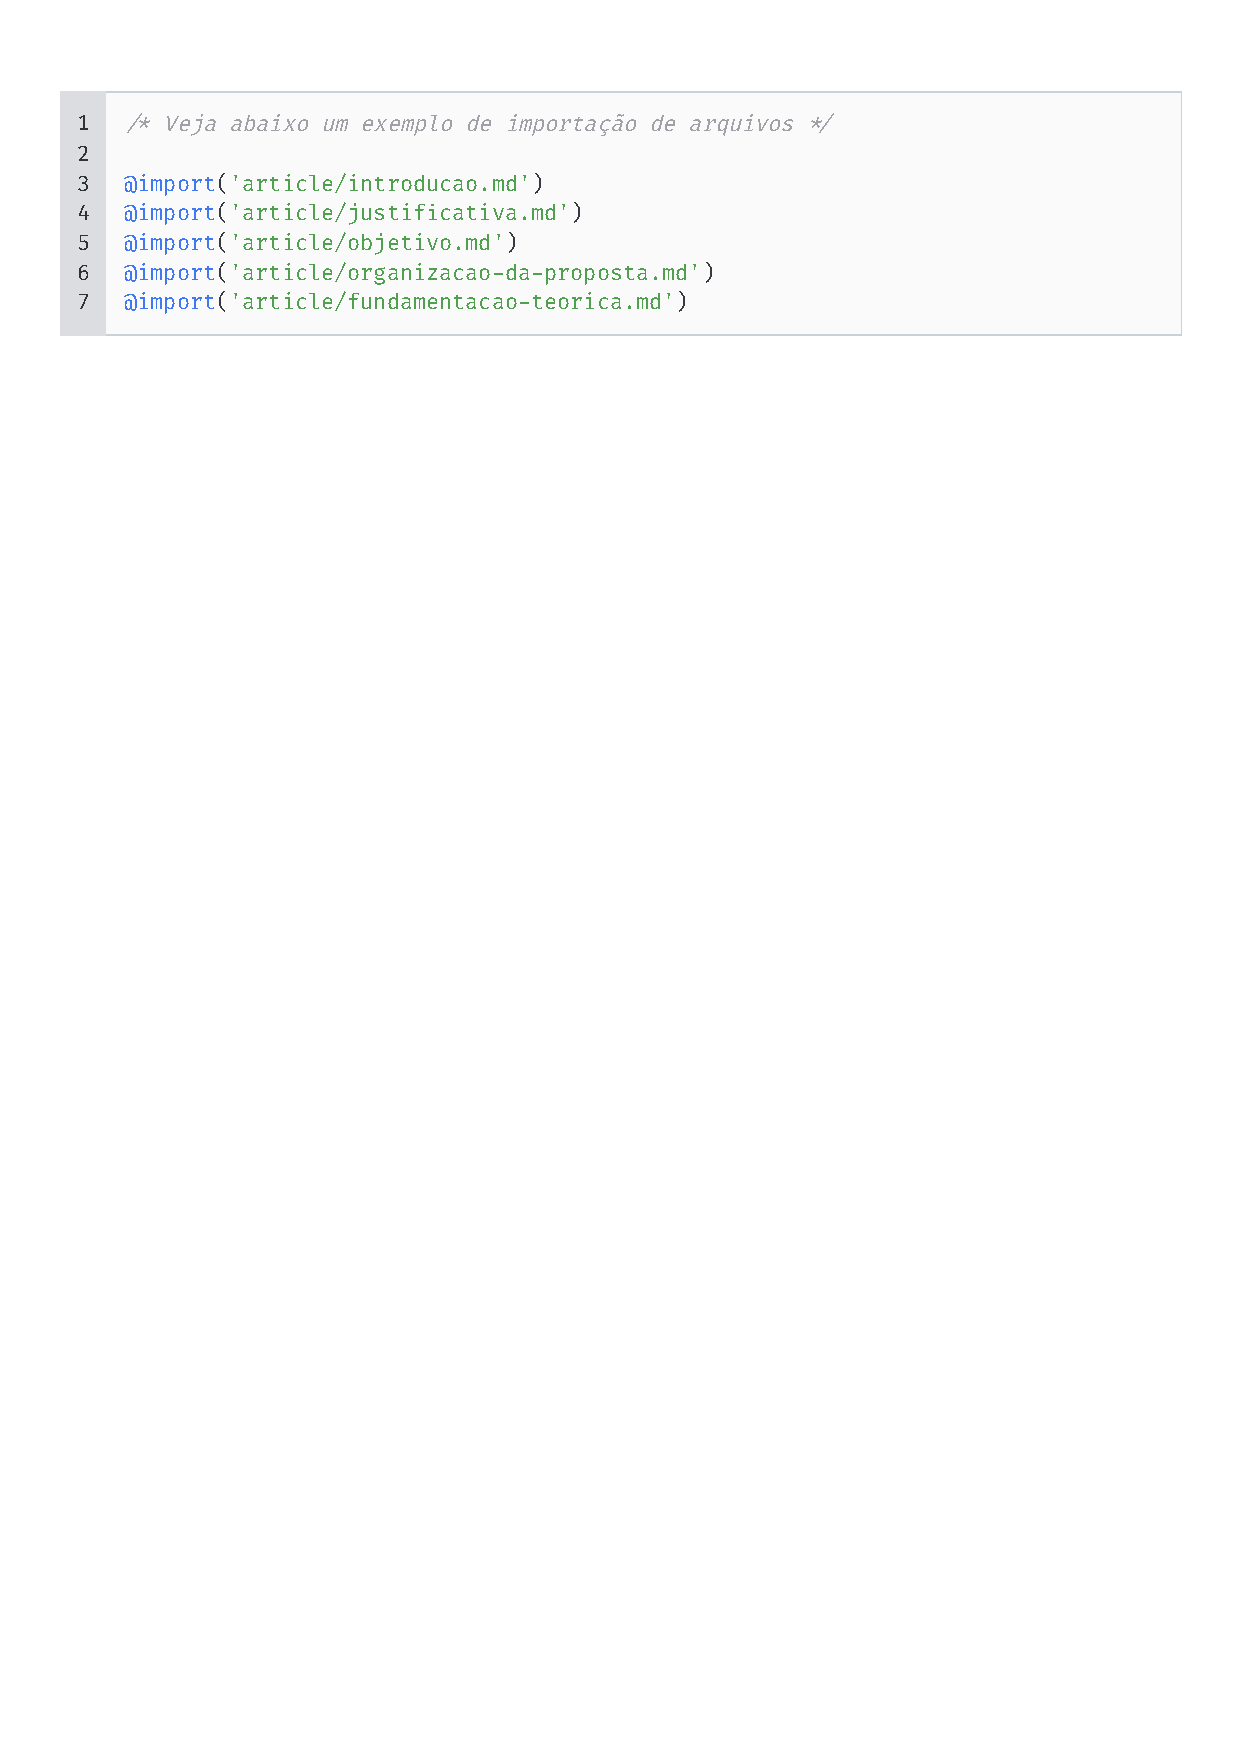
\includegraphics[scale=0.8]{imagens/code/markdown-import-code.pdf}
\end{center}
}
\legend{Fonte: Autor.}
\end{figure}

Ao aplicar essa estratégia de importação de arquivos Markdown no modelo
original, diversos benefícios são proporcionados aos usuários do
Limarka. A escrita modular e a organização aprimorada tornam o processo
de elaboração de TCCs mais eficiente e menos propenso a erros. Além
disso, a facilidade de colaboração e a clareza na estrutura do projeto
contribuem para uma melhor experiência de uso.

\hypertarget{reposituxf3rio-docker}{%
\section{Repositório Docker}\label{reposituxf3rio-docker}}

Para implementar as funcionalidades necessárias para a organização de
pastas e importação de arquivos, foi necessário adicionar algumas
customizações na imagem original da ferramenta Limarka. Essas
customizações visavam garantir que a ferramenta suportasse as novas
funcionalidades e fornecesse um ambiente consistente e atualizado para
os usuários. Diante dessa necessidade, foi criado um repositório Docker
específico para gerenciar essas modificações.

\hypertarget{criauxe7uxe3o-e-automauxe7uxe3o-do-reposituxf3rio-limarka-docker}{%
\subsection{Criação e automação do repositório
limarka-docker}\label{criauxe7uxe3o-e-automauxe7uxe3o-do-reposituxf3rio-limarka-docker}}

O repositório
\href{https://github.com/ReinanHS/limarka-docker}{limarka-docker} foi
criado com o propósito de facilitar a manutenção e atualização das
imagens Docker utilizadas pelo Limarka. Essa iniciativa permitiu a
personalização do ambiente de desenvolvimento e execução, incorporando
todas as dependências e configurações necessárias para suportar as novas
funcionalidades implementadas.

Para garantir que as imagens Docker estivessem sempre atualizadas, foi
automatizado o processo de construção e publicação das imagens. A
automação foi configurada para gerar novas versões das imagens sempre
que mudanças fossem feitas no repositório, garantindo que as melhorias e
correções fossem rapidamente disponibilizadas aos usuários.

\hypertarget{atualizauxe7uxf5es-de-seguranuxe7a-e-publicauxe7uxe3o-no-docker-hub}{%
\subsection{Atualizações de segurança e publicação no Docker
Hub}\label{atualizauxe7uxf5es-de-seguranuxe7a-e-publicauxe7uxe3o-no-docker-hub}}

Manter as imagens Docker atualizadas é crucial para garantir a segurança
e a estabilidade da ferramenta. No repositório
\href{https://github.com/ReinanHS/limarka-docker}{limarka-docker}, foram
implementadas automatizações que verificam e aplicam atualizações de
segurança regularmente. Isso assegura que as imagens Docker estejam
sempre protegidas contra vulnerabilidades e utilizem as versões mais
recentes dos pacotes e dependências.

Além disso, as imagens Docker são publicadas no Docker Hub, facilitando
o acesso e a utilização por parte dos alunos. A publicação no Docker Hub
permite que as imagens sejam facilmente integradas em diferentes
ambientes de desenvolvimento, tornando a configuração e o uso do Limarka
mais acessíveis e eficientes.

\hypertarget{integrauxe7uxe3o-das-imagens-docker-no-limarka-template-tcc}{%
\subsection{Integração das imagens Docker no
limarka-template-tcc}\label{integrauxe7uxe3o-das-imagens-docker-no-limarka-template-tcc}}

A integração das imagens Docker no
\href{https://github.com/ReinanHS/limarka-template-tcc}{limarka-template-tcc}
foi uma etapa crucial para garantir a consistência e a funcionalidade
das novas melhorias implementadas. Utilizando as imagens Docker
personalizadas, os alunos podem configurar rapidamente seu ambiente de
desenvolvimento e execução, aproveitando todas as vantagens das novas
funcionalidades sem a necessidade de configurações complexas.

Essa integração também garante que todos os usuários estejam utilizando
a mesma versão da ferramenta, minimizando problemas de compatibilidade e
facilitando a colaboração. A utilização das imagens Docker atualizadas e
personalizadas assegura que o ambiente de desenvolvimento esteja sempre
alinhado com as últimas melhorias e correções, proporcionando uma
experiência de uso mais suave e eficiente.

\hypertarget{integrauxe7uxe3o-com-github-codespaces}{%
\section{Integração com GitHub
Codespaces}\label{integrauxe7uxe3o-com-github-codespaces}}

A integração do
\href{https://github.com/ReinanHS/limarka-template-tcc}{limarka-template-tcc}
com o GitHub Codespaces foi uma etapa estratégica para tornar o
desenvolvimento e a escrita de trabalhos acadêmicos ainda mais
acessíveis e eficientes. O GitHub Codespaces oferece um ambiente de
desenvolvimento completo no navegador, eliminando a necessidade de
configurações locais.

\hypertarget{configurauxe7uxe3o-do-template-para-uso-no-github-codespaces}{%
\subsection{Configuração do template para uso no GitHub
Codespaces}\label{configurauxe7uxe3o-do-template-para-uso-no-github-codespaces}}

Para configurar o
\href{https://github.com/ReinanHS/limarka-template-tcc}{limarka-template-tcc}
para uso no GitHub Codespaces, foram realizadas diversas adaptações no
projeto. Primeiramente, foi necessário criar um diretório
\texttt{.devcontainer} contendo os arquivos de configuração necessários
para definir o ambiente de desenvolvimento.

Os arquivos de configuração no \texttt{.devcontainer} especificam a
imagem Docker personalizada, garantindo que o ambiente de
desenvolvimento no Codespaces seja idêntico ao utilizado localmente. A
Figura \ref{devcontainer_config_json} apresenta um exemplo da
configuração para o GitHub Codespaces:

\begin{figure}[htbp]
\hypertarget{devcontainer_config_json}{%
\caption{Exemplo da configuração para o GitHub Codespaces}\label{devcontainer_config_json}
\begin{center}
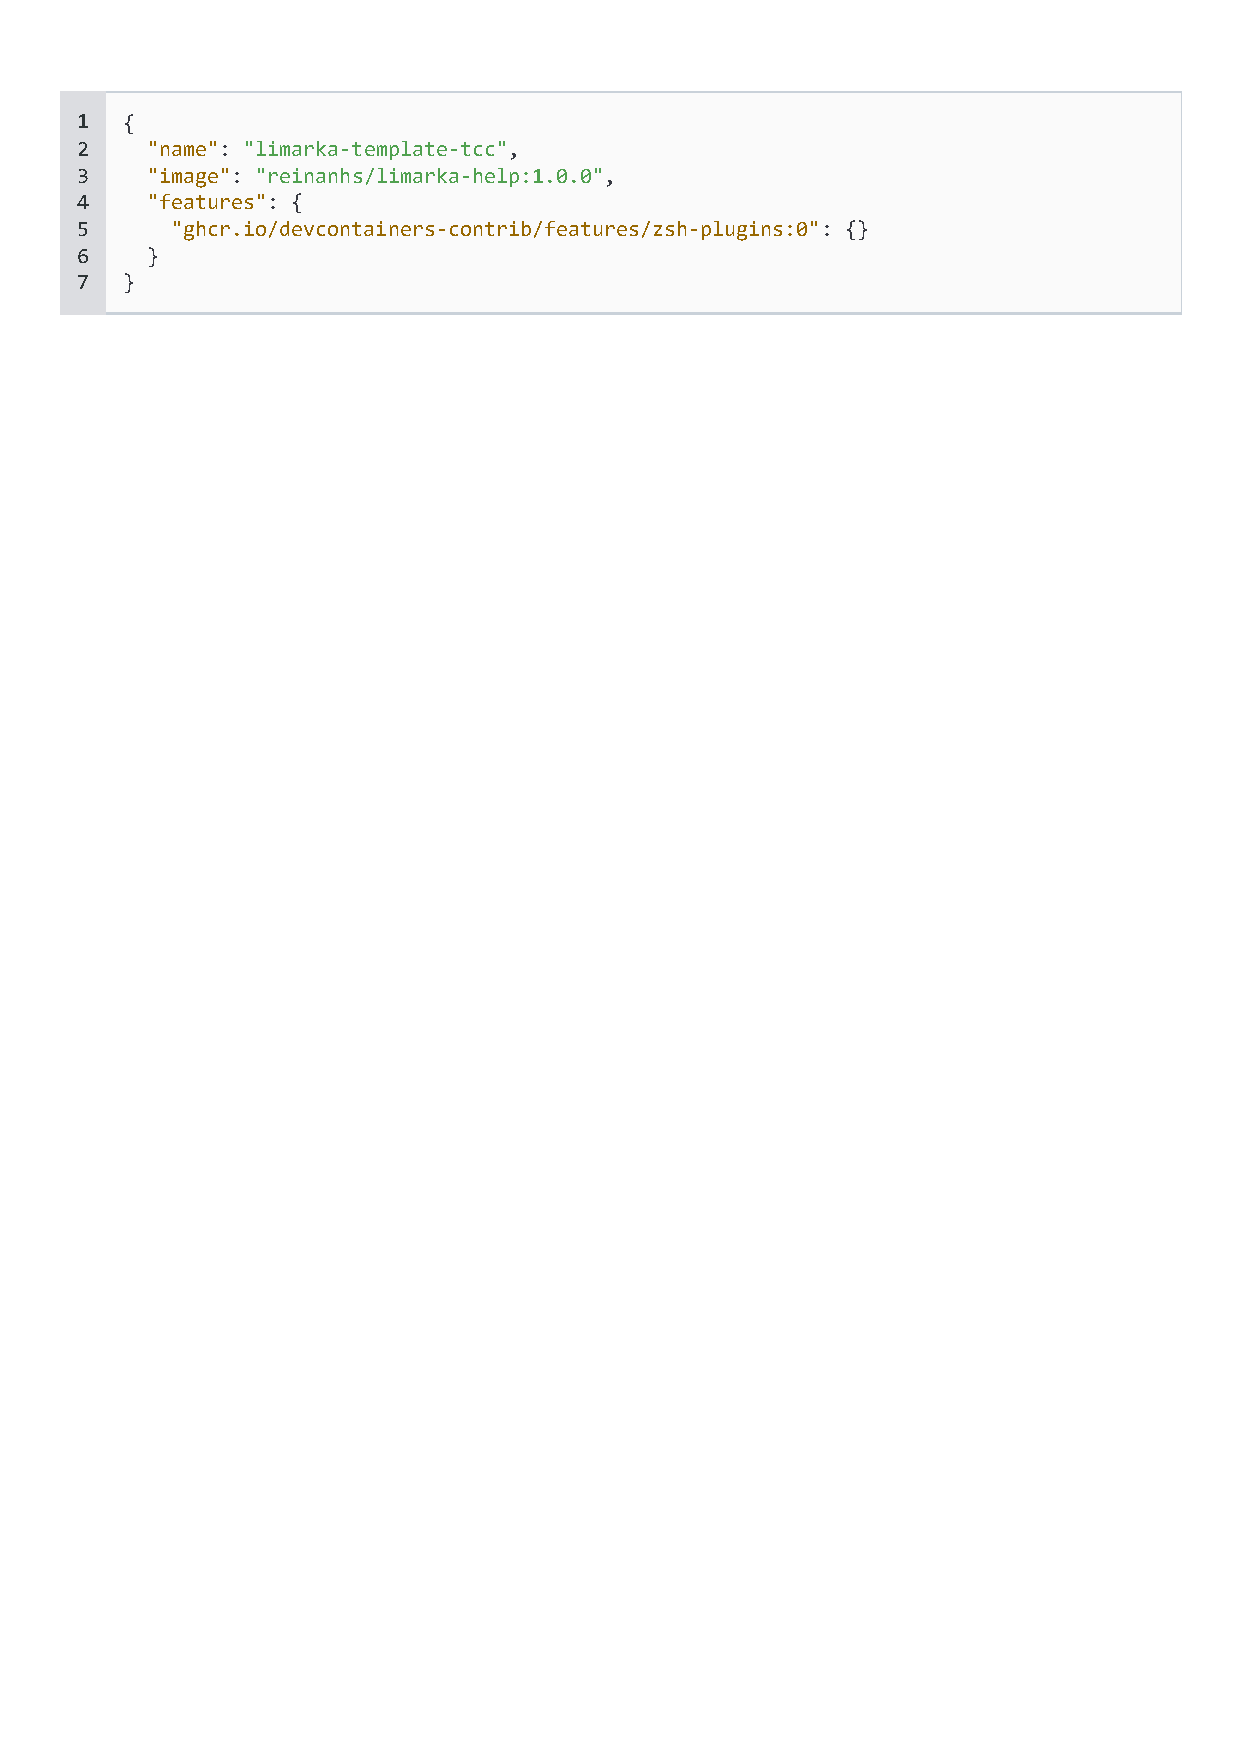
\includegraphics[scale=0.8]{imagens/code/devcontainer-config-json.pdf}
\end{center}
}
\legend{Fonte: Autor.}
\end{figure}

Ao analisar a configuração, é possível observar que há uma referência à
imagem criada no repositório Docker, na qual foram realizadas
customizações para implementar as funcionalidades do novo modelo. Esse
tipo de referência assegura que os alunos utilizem um ambiente já
equipado com as ferramentas necessárias para executar o Limarka. Além
disso, foram configurados scripts de inicialização que automatizam a
configuração inicial, incluindo a instalação de extensões essenciais
para o funcionamento do Limarka.

\hypertarget{devops-e-automauxe7uxe3o}{%
\section{DevOps e automação}\label{devops-e-automauxe7uxe3o}}

A implementação de práticas de DevOps e automação foi essencial para
aprimorar o fluxo de trabalho do projeto Limarka, tornando o processo de
geração de documentos acadêmicos mais eficiente e robusto. Para alcançar
esses objetivos, foram utilizadas pipelines no GitHub Actions, que
automatizam tarefas críticas como a validação de arquivos Markdown, a
geração de PDFs e a publicação de páginas HTML. A Figura
\ref{github_action_limarka} ilustra o fluxo de execução da pipeline no
GitHub Actions:

\begin{figure}[htbp]
\hypertarget{github_action_limarka}{%
\caption{Exemplificação do fluxo de execução da pipeline}\label{github_action_limarka}
\begin{center}
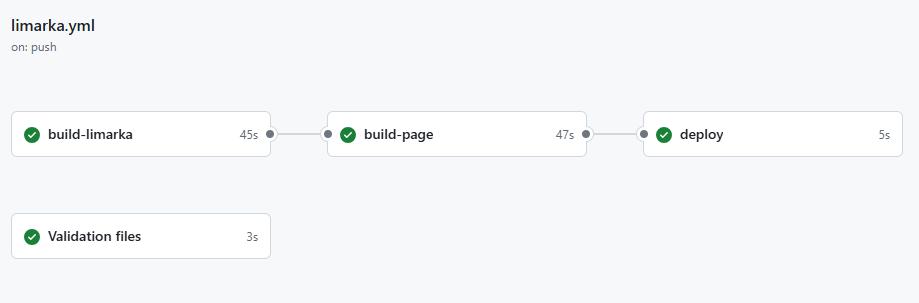
\includegraphics[scale=0.6]{imagens/screenshot/github-action-limarka.png}
\end{center}
}
\legend{Fonte: Autor.}
\end{figure}

Com a compilação gerada por uma pipeline, os alunos podem ter seus
documentos constantemente atualizados e publicados no GitHub Pages. Isso
garante que a página HTML gerada contenha sempre o conteúdo mais
atualizado disponível no repositório do GitHub.

\hypertarget{implementauxe7uxe3o-da-pipeline-no-github-actions}{%
\subsection{Implementação da Pipeline no GitHub
Actions}\label{implementauxe7uxe3o-da-pipeline-no-github-actions}}

A configuração da pipeline no GitHub Actions foi projetada para garantir
a consistência e a qualidade dos documentos gerados pelo Limarka. A
pipeline é acionada automaticamente sempre que há um push na branch
\texttt{master}, iniciando uma série de jobs que verificam e processam o
conteúdo do repositório.

\hypertarget{validauxe7uxe3o-dos-arquivos-markdown}{%
\subsubsection{Validação dos arquivos
Markdown}\label{validauxe7uxe3o-dos-arquivos-markdown}}

O primeiro job, denominado \texttt{markdown-lint}, é responsável pela
validação dos arquivos Markdown no repositório. Utilizando a ação
\texttt{DavidAnson/markdownlint-cli2-action}, o job verifica se os
arquivos Markdown estão em conformidade com as regras de formatação
especificadas no arquivo \texttt{.markdownlint.yml}. Esta etapa é
crucial para garantir a qualidade e a consistência do conteúdo antes de
prosseguir para a compilação. A Figura \ref{markdown_lint_code} tem o
exemplo do código em YAML para a configuração da job:

\begin{figure}[htbp]
\hypertarget{markdown_lint_code}{%
\caption{Exemplo do bloco de código do markdown-lint}\label{markdown_lint_code}
\begin{center}
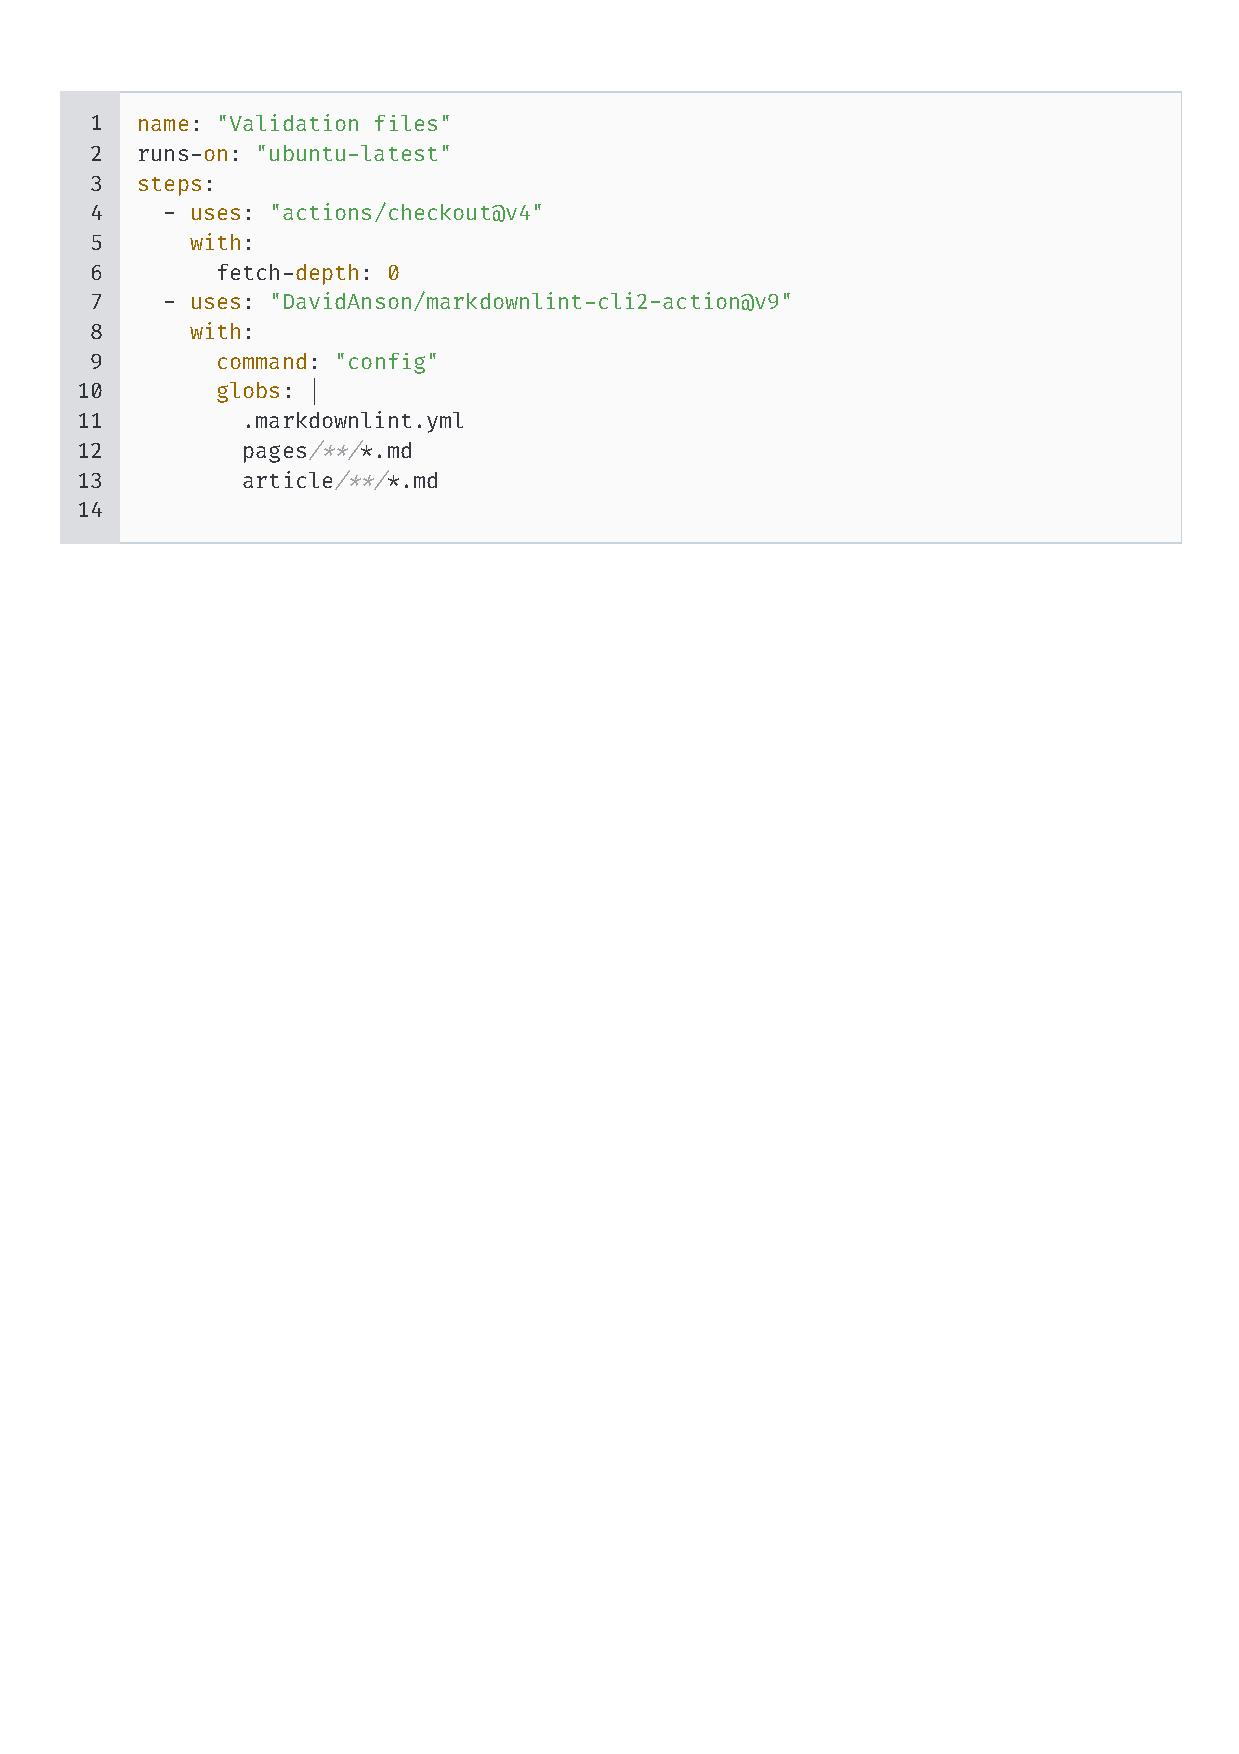
\includegraphics[scale=0.8]{imagens/code/markdown-lint-code.pdf}
\end{center}
}
\legend{Fonte: Autor.}
\end{figure}

\hypertarget{compilauxe7uxe3o-do-documento-com-limarka}{%
\subsubsection{Compilação do documento com
Limarka}\label{compilauxe7uxe3o-do-documento-com-limarka}}

O segundo job, \texttt{build-limarka}, realiza a compilação do documento
utilizando a imagem Docker personalizada
\texttt{reinanhs/limarka-help:1.0.0}. Este job executa comandos para
verificar e compilar o documento, movendo os arquivos gerados para um
diretório específico (\texttt{dist}). A etapa final deste job envolve o
upload dos artefatos compilados para que possam ser utilizados em etapas
subsequentes.

\hypertarget{gerauxe7uxe3o-automuxe1tica-do-pdf-e-publicauxe7uxe3o-no-github-pages}{%
\subsubsection{Geração automática do PDF e publicação no GitHub
Pages}\label{gerauxe7uxe3o-automuxe1tica-do-pdf-e-publicauxe7uxe3o-no-github-pages}}

Após a compilação do documento, a próxima etapa envolve a geração de uma
página HTML e a publicação do conteúdo no GitHub Pages. Este processo é
gerido por dois jobs: \texttt{build-page} e \texttt{deploy}.

O job \texttt{build-page} depende da conclusão bem-sucedida do job
\texttt{build-limarka}. Ele baixa os artefatos compilados e utiliza o
\texttt{limarka-render-html} para gerar a versão HTML do documento. A
estrutura HTML é então preparada para ser publicada, garantindo que
todas as partes do documento estejam corretamente formatadas e prontas
para visualização na web.

O job final de \texttt{deploy} realiza a publicação do conteúdo gerado
no GitHub Pages. Utilizando a action
\texttt{JamesIves/github-pages-deploy-action}, esse job faz o deploy do
diretório build para o GitHub Pages, tornando o documento acadêmico
acessível pela internet. Esta etapa garante que a versão mais recente do
documento esteja sempre disponível para visualização pública,
facilitando o acesso e a disseminação do trabalho acadêmico.

\hypertarget{documentauxe7uxe3o-1}{%
\section{Documentação}\label{documentauxe7uxe3o-1}}

Para facilitar o uso da ferramenta pelos alunos, a documentação original
foi reescrita utilizando a metodologia Doc as Code. Essa abordagem
garante que a documentação esteja sempre atualizada em relação ao modelo
de template. Além disso, a nova documentação orienta os alunos sobre
como utilizar os novos recursos implementados no modelo atualizado do
template.

A documentação criada fornece referências abrangentes para todas as
funcionalidades disponíveis na ferramenta, além de orientações sobre
como configurar a ferramenta em diversos tipos de ambientes. A Figura
\ref{limarka_template_docs} exemplifica a página da documentação
disponível no
\href{https://reinanhs.github.io/limarka-template-docs}{GitHub Pages}.

\begin{figure}[htbp]
\hypertarget{limarka_template_docs}{%
\caption{Demonstração da página da documentação}\label{limarka_template_docs}
\begin{center}
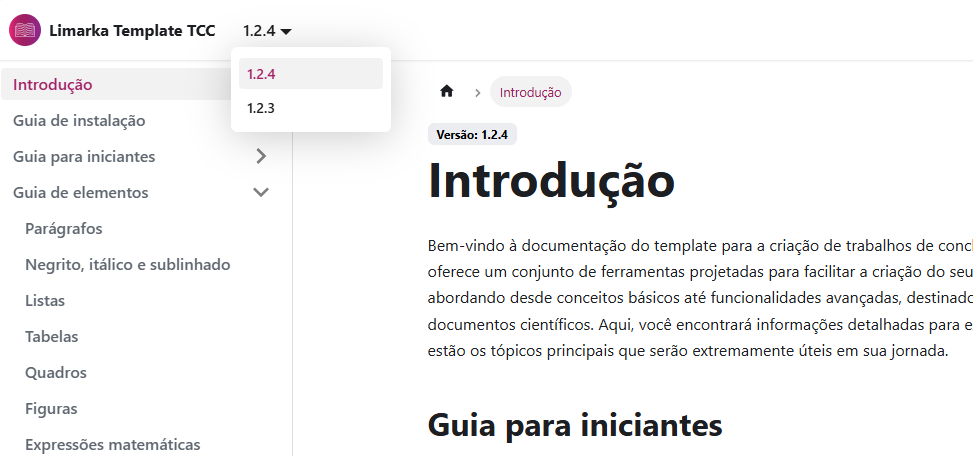
\includegraphics[scale=0.6]{imagens/screenshot/limarka-template-docs.png}
\end{center}
}
\legend{Fonte: Autor.}
\end{figure}

Ao acessar o
\href{https://reinanhs.github.io/limarka-template-docs}{site da
documentação}, os alunos encontrarão informações detalhadas sobre
diversas funcionalidades da ferramenta. Além disso, a documentação
possui um sistema de versionamento que acompanha a versão do repositório
do GitHub do modelo. Isso garante que, se o modelo for atualizado ou uma
funcionalidade for descontinuada, essas mudanças serão refletidas apenas
na versão correspondente da documentação. As versões antigas continuarão
oferecendo suporte e orientações sobre como a ferramenta era utilizada
em versões anteriores.

\hypertarget{metodologia-doc-as-code}{%
\subsection{Metodologia Doc as Code}\label{metodologia-doc-as-code}}

A metodologia Doc as Code é um paradigma que trata a documentação do
software com a mesma importância e as mesmas práticas utilizadas no
desenvolvimento de código. Isso significa que a documentação é escrita
em formato de texto simples, como Markdown, e armazenada no controle de
versão junto com o código-fonte. A documentação é gerida e atualizada
usando as mesmas ferramentas e processos de desenvolvimento, como
revisões de código, testes automatizados e integração contínua. Essa
abordagem garante que a documentação evolua simultaneamente com o
código, mantendo-se sempre relevante e precisa.

\hypertarget{criauxe7uxe3o-do-reposituxf3rio-limarka-template-docs}{%
\subsubsection{Criação do Repositório
limarka-template-docs}\label{criauxe7uxe3o-do-reposituxf3rio-limarka-template-docs}}

Para implementar a filosofia da documentação como código de forma mais
eficaz, foi criado o repositório \texttt{limarka-template-docs} no
GitHub para gerenciar a publicação da documentação. Esse repositório
segue a estrutura da ferramenta Docusaurus, uma solução popular para a
geração de sites estáticos e de documentação. Com isso, foi criado o
layout da documentação e configurada a sincronização da pasta de
documentação do
\href{https://github.com/ReinanHS/limarka-template-tcc}{repositório
principal} com esse repositório.

Essa sincronização é realizada através das versões publicadas,
permitindo que a ferramenta baixe a versão, compile a documentação
específica e a mescle com o layout presente nesse repositório. Após esse
processo, a documentação é publicada no GitHub Pages. A figura
\ref{limarka_template_docs_ci_cd} exemplifica o fluxo de execução do
CI/CD nesse repositório:

\begin{figure}[htbp]
\hypertarget{limarka_template_docs_ci_cd}{%
\caption{Demonstração do CI/CD para o limarka-template-docs}\label{limarka_template_docs_ci_cd}
\begin{center}
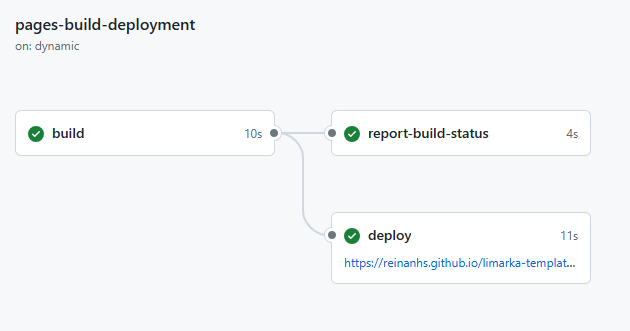
\includegraphics[scale=0.6]{imagens/screenshot/limarka-template-docs-ci-cd.png}
\end{center}
}
\legend{Fonte: Autor.}
\end{figure}

Ao observar a imagem, é possível perceber que as informações são
compiladas e processadas antes de serem publicadas na página do GitHub
Pages. Isso garante que os alunos sempre encontrarão a documentação
atualizada e consistente com o repositório principal.

\hypertarget{vantagens-de-manter-a-documentauxe7uxe3o-atualizada-junto-com-o-cuxf3digo}{%
\subsubsection{Vantagens de manter a documentação atualizada junto com o
código}\label{vantagens-de-manter-a-documentauxe7uxe3o-atualizada-junto-com-o-cuxf3digo}}

Manter a documentação atualizada junto com o código oferece vários
benefícios significativos para os alunos. Primeiramente, essa abordagem
assegura que a documentação reflete as mudanças mais recentes no código,
proporcionando aos alunos informações precisas e atualizadas sobre o uso
da ferramenta. Isso elimina a frustração de seguir instruções
desatualizadas e permite que os alunos aproveitem plenamente as últimas
melhorias e correções.

Além disso, a documentação integrada com o ciclo de desenvolvimento
facilita a aprendizagem contínua. À medida que novos recursos são
adicionados ou modificados, os alunos podem acessar rapidamente a
documentação relevante, sem necessidade de esperar por atualizações
manuais. Essa sincronia entre código e documentação melhora a eficiência
no aprendizado e na aplicação prática da ferramenta, garantindo uma
experiência de usuário mais coesa e satisfatória.

\hypertarget{aspectos-cobertos-pela-documentauxe7uxe3o}{%
\subsection{Aspectos cobertos pela
documentação}\label{aspectos-cobertos-pela-documentauxe7uxe3o}}

A nova documentação que foi feita é abrangente e cobre todos os aspectos
necessários para garantir que os usuários, desde iniciantes até
colaboradores avançados, possam utilizar e contribuir com a ferramenta
de forma eficiente. Ela está organizada em seções específicas que
abordam desde a instalação inicial até funcionalidades avançadas, com
exemplos práticos que facilitam o entendimento e a aplicação dos
conceitos. A seguir, detalhamos os principais guias incluídos na
documentação, cada um com seu foco particular para atender às
necessidades de diferentes tipos de usuários.

\hypertarget{guia-de-instalauxe7uxe3o}{%
\subsubsection{Guia de instalação}\label{guia-de-instalauxe7uxe3o}}

Para ajudar os alunos a instalarem a ferramenta Limarka, foi criada uma
seção abrangente denominada guia de instalação. Este guia visa
proporcionar aos novos usuários uma compreensão completa de como
configurar o Limarka em diferentes sistemas operacionais e ambientes de
desenvolvimento. Além disso, foram desenvolvidos casos práticos de uso,
mostrando exemplos reais de instalação e configuração.

A introdução à instalação oferece uma visão geral dos passos necessários
para configurar o Limarka, garantindo que todos os requisitos sejam
atendidos. São listadas as dependências essenciais como Docker, além de
orientações sobre como instalá-las.

Para usuários do GitHub Codespace, o guia mostra como configurar
rapidamente um ambiente de desenvolvimento no navegador, sem a
necessidade de instalar nada localmente. São fornecidos passos
detalhados para fazer um fork do repositório, configurar o Codespace e
verificar a instalação do Limarka, garantindo que tudo esteja
funcionando corretamente.

No Linux, o guia orienta os usuários pela instalação das dependências e
do próprio Limarka. Os passos incluem a instalação do Docker. Exemplos
práticos são fornecidos para verificar a instalação e realizar uma
compilação de teste.

Para usuários do macOS, o guia detalha como utilizar o Homebrew para
instalar as dependências necessárias. São fornecidos passos claros para
configurar o ambiente e garantir que o Limarka esteja instalado
corretamente. Exemplos práticos demonstram como verificar a instalação e
compilar um documento.

No Windows, o guia aborda os passos adicionais necessários. São
fornecidas instruções para a instalação do Docker. Exemplos práticos
ajudam a verificar a instalação e realizar uma compilação de teste.

\hypertarget{guia-para-iniciantes}{%
\subsubsection{Guia para iniciantes}\label{guia-para-iniciantes}}

Para ajudar os alunos a iniciarem o uso da ferramenta Limarka, foi
criada uma seção abrangente denominada guia para iniciantes. Este guia
visa proporcionar aos novos usuários uma compreensão completa de como
configurar, utilizar e compilar documentos com o Limarka. Além disso,
foram desenvolvidos casos práticos de uso, mostrando exemplos reais de
configurações e compilações.

O guia aborda a configuração inicial do Limarka, um passo essencial para
garantir um ambiente de trabalho adequado. Os alunos são orientados
sobre a instalação das dependências necessárias, clonagem do repositório
e configuração dos arquivos essenciais, como o
\texttt{configuracao.yaml}. Exemplos práticos são fornecidos para
demonstrar como definir corretamente as opções do template, garantindo
que todas as informações do TCC estejam bem configuradas.

A seção de compilação detalha como transformar o documento Markdown em
um PDF formatado de acordo com as normas acadêmicas. O guia explica os
passos necessários, desde a preparação do ambiente até a execução do
comando \texttt{limarka\ build} para iniciar a compilação. Exemplos
práticos ilustram o processo de criação de um documento simples e sua
transformação em PDF.

O guia também apresenta o Playground, um ambiente de testes onde os
alunos podem experimentar diferentes configurações e funcionalidades do
Limarka sem afetar o projeto principal. As instruções mostram como criar
um ambiente de testes, testar diferentes configurações e elementos de
Markdown, e compilar os arquivos para verificar os resultados. Exemplos
práticos demonstram como utilizar o Playground para experimentar com
segurança.

\hypertarget{guia-de-elementos}{%
\subsubsection{Guia de elementos}\label{guia-de-elementos}}

Para ajudar os alunos a entender os elementos que a ferramenta Limarka
dispõe, foi criada uma seção abrangente denominada guia de elementos.
Este guia visa proporcionar aos alunos uma compreensão completa de todos
os componentes disponíveis na ferramenta e como utilizá-los de maneira
eficaz. Além disso, foram desenvolvidos casos práticos de uso, mostrando
exemplos reais e como esses elementos se comportam após a compilação.

O guia aborda os parágrafos, que são a base de qualquer documento
textual. Detalha como criar parágrafos bem estruturados no Limarka
utilizando Markdown, garantindo clareza e coesão no texto. Exemplos
práticos são fornecidos para demonstrar a criação de parágrafos simples
e eficazes.

Também são discutidos os quadros, utilizados para destacar informações
importantes ou fornecer exemplos detalhados. O guia oferece instruções
sobre como criar quadros usando Markdown e HTML. Casos práticos ilustram
como os quadros podem ser usados para organizar e apresentar dados de
maneira clara.

A seção sobre tabelas ensina como criar tabelas utilizando a sintaxe
Markdown, essenciais para a organização de dados de forma estruturada.
Exemplos mostram a construção e formatação de tabelas para diferentes
tipos de dados, e casos práticos demonstram sua aplicação em contextos
acadêmicos.

No que diz respeito à citação de fontes, o guia explica como gerenciar
bibliografias e referências utilizando Markdown e BibTeX, com exemplos
detalhados de como citar fontes no texto e adicionar referências
bibliográficas. Casos práticos evidenciam a importância de seguir os
padrões acadêmicos.

As figuras, que são elementos visuais que complementam o texto e
enriquecem o conteúdo do documento, também são cobertas. O guia fornece
instruções sobre como inserir figuras utilizando a sintaxe Markdown, com
exemplos que ilustram a adição de imagens e sua formatação adequada.
Casos práticos mostram como figuras podem ser integradas ao texto para
melhor compreensão.

Para organizar informações de maneira clara e fácil de ler, o guia
explica como criar listas ordenadas e não ordenadas utilizando Markdown.
Exemplos práticos mostram a criação e formatação de listas para diversos
tipos de conteúdo.

Além disso, o guia detalha como escrever fórmulas em LaTeX e inseri-las
diretamente no Markdown, com exemplos que demonstram a criação de
equações complexas. Casos práticos mostram a aplicação das fórmulas em
contextos científicos.

\hypertarget{guias-avanuxe7ados}{%
\subsubsection{Guias avançados}\label{guias-avanuxe7ados}}

Para ajudar os alunos e colaboradores a explorarem mais a fundo as
capacidades do Limarka, foi criada uma seção abrangente denominada guias
avançados. Este guia visa proporcionar uma compreensão detalhada de
aspectos complexos do Limarka, como a arquitetura do template, a geração
de sites estáticos e como contribuir para o projeto. Além disso, foram
desenvolvidos casos práticos de uso, mostrando exemplos reais e como
aplicar essas funcionalidades.

A seção sobre a arquitetura do template detalha a organização interna do
projeto Limarka para trabalhos de conclusão de curso (TCC). Os alunos e
colaboradores encontram uma descrição completa dos arquivos e diretórios
que compõem o projeto, facilitando a compreensão da estrutura e a
localização dos componentes. Isso é fundamental para quem deseja
modificar, personalizar ou contribuir para o projeto. Exemplos práticos
e uma árvore do projeto ajudam a visualizar e entender a organização do
template.

A geração de sites estáticos é outra funcionalidade avançada abordada no
guia. Este segmento da documentação explica como o Limarka integra
automação de CI/CD para compilar o projeto e transformá-lo em um site
estático em HTML, tornando-o acessível pela internet. São fornecidos
detalhes sobre a configuração do arquivo destinado à geração de conteúdo
estático, personalização das páginas HTML e implantação no GitHub Pages.
Casos práticos ilustram o processo de configuração e publicação,
promovendo uma forma inovadora e eficaz de compartilhar documentos
acadêmicos online.

Por fim, o guia aborda como contribuir para o projeto, enfatizando a
importância da colaboração para o desenvolvimento e aprimoramento de
projetos de código aberto. Os alunos e colaboradores encontram
informações sobre pré-requisitos para contribuição, como familiarizar-se
com Git e a documentação do projeto, além de seguir o código de conduta.
Instruções detalhadas mostram como criar um fork do repositório, clonar
o fork, criar uma branch, fazer alterações, commit e push das mudanças,
e finalmente, criar um pull request. Casos práticos e exemplos guiam os
novos contribuidores através do processo, incentivando a participação
ativa na comunidade do Limarka.

\hypertarget{cronograma-de-atividades}{%
\chapter{Cronograma de Atividades}\label{cronograma-de-atividades}}

\hypertarget{atividades-realizadas}{%
\section{Atividades realizadas}\label{atividades-realizadas}}

\hypertarget{atividades-previstas}{%
\section{Atividades previstas}\label{atividades-previstas}}

\hypertarget{cronograma}{%
\section{Cronograma}\label{cronograma}}

% ----------------------------------------------------------
% ELEMENTOS PÓS-TEXTUAIS
% ----------------------------------------------------------
\postextual
% ----------------------------------------------------------

% ----------------------------------------------------------
% Início dos ELEMENTOS PÓS-TEXTUAIS
% ----------------------------------------------------------
\postextual
% ----------------------------------------------------------

% ----------------------------------------------------------
% Referências bibliográficas
% ----------------------------------------------------------
\bibliography{xxx-referencias}
% ----------------------------------------------------------
% Apêndices
% ----------------------------------------------------------
%% 
% Seção de apendices configurada como desativada
%% 
% ---

% ----------------------------------------------------------
% Anexos desativados: 
% Seção de anexos configurada como desativada
% ----------------------------------------------------------



\end{document}
